\documentclass[aspectratio=169,10pt]{beamer}

\usetheme[progressbar=frametitle,numbering=fraction,sectionpage=none]{metropolis}
\usepackage[utf8]{inputenc}
\usepackage[T1]{fontenc}
\usepackage{lmodern}
\usepackage{amsmath,amssymb}
\usepackage{booktabs}
\usepackage{array}
\newcolumntype{L}[1]{>{\raggedright\arraybackslash}p{#1}}
\usepackage{graphicx}
\usepackage{tikz}
\usetikzlibrary{positioning,arrows.meta,fit,backgrounds,calc}
\graphicspath{{figures/}}

% ---- restrained palette ----
\definecolor{ink}{HTML}{1F2937}
\definecolor{accent}{HTML}{2563EB}
\definecolor{warm}{HTML}{C2410C}
\definecolor{good}{HTML}{047857}
\definecolor{soft}{HTML}{EEF2F7}
\setbeamercolor{frametitle}{bg=ink,fg=white}
\setbeamercolor{progress bar}{fg=accent,bg=soft}
\setbeamercolor{alerted text}{fg=warm}
\setbeamercolor{example text}{fg=good}
\setbeamercolor{block title}{bg=soft,fg=ink}
\setbeamercolor{block body}{bg=soft!40}
\setbeamerfont{caption}{size=\scriptsize}
\setbeamerfont{title}{size=\large}
\setbeamerfont{subtitle}{size=\small}

% metropolis' title page uses a \paperheight-tall minipage, which overflows by ~14pt; shorten it
\makeatletter
\setbeamertemplate{title page}{
  \begin{minipage}[b][\dimexpr\paperheight-16pt\relax]{\textwidth}
    \vfill%
    \ifx\inserttitle\@empty\else\usebeamertemplate*{title}\fi
    \ifx\insertsubtitle\@empty\else\usebeamertemplate*{subtitle}\fi
    \usebeamertemplate*{title separator}
    \ifx\beamer@shortauthor\@empty\else\usebeamertemplate*{author}\fi
    \ifx\insertdate\@empty\else\usebeamertemplate*{date}\fi
    \vfill
    \vspace*{1mm}
  \end{minipage}
}
\makeatother

\newcommand{\pilot}{\textcolor{warm}{\textbf{[pilot]}}}
\newcommand{\illus}{\textcolor{warm}{\textbf{[illustrative, untrained]}}}
\newcommand{\snote}[1]{{\scriptsize\textcolor{ink!70}{#1}}}

\title{Mechanistic Analysis of Over-Squashing and Attention Dilution in Hybrid GNNs}
\subtitle{Problem, data, replications, pipeline, measures and first results}
\author{MS Applied Data Science capstone}
\date{October 2026}

\begin{document}

\maketitle

\begin{frame}{Outline}
  \setbeamertemplate{section in toc}[sections numbered]
  \tableofcontents
\end{frame}

% =====================================================================
\section{Problem overview}


\begin{frame}{Over-squashing: Jacobian decay and resistance bottlenecks}
  \begin{itemize}
    \item Bottlenecks compress information from many nodes \snote{(Alon \& Yahav 2021; Topping et al. 2022)}
    \item Measured by the sensitivity of a node's output to a distant input:
      \[ J(u,v) = \Big\|\frac{\partial h_v^{(L)}}{\partial h_u^{(0)}}\Big\|_F \quad\text{decays with distance} \]
    \item Depends on width, depth and topology \snote{(Di Giovanni et al. 2023)}
    \item Structural predictor: \textbf{effective resistance} $R(u,v)$; total resistance bounds over-squashing \snote{(Black et al. 2023)}
    \item On trees $R(u,v)$ equals the hop distance
  \end{itemize}
\end{frame}

\begin{frame}{Attention dilution: entropy $\to \log N$, sensitivity $\sim 1/N$}
  \begin{itemize}
    \item Global softmax attention: row $a_{i\cdot}$ is a distribution over $N$ nodes
    \item Uninformative attention is uniform: entropy $H = \log N$, so each source has weight $1/N$
    \item Diagnostic: per-head entropy normalised by $\log N$
      \[ \tilde H = H/\log N \in [0,1],\qquad \tilde H \approx 1 \;\Rightarrow\; \text{attention fails to concentrate} \]
    \item Dilution in a \emph{trained} model: $\tilde H$ stays near 1 as $N$ grows
    \item Raw $H$ rising with $N$ is automatic and is not, by itself, evidence of dilution
  \end{itemize}
\end{frame}

\begin{frame}{The hybrid idea: an $\alpha$-blend per layer}
  \[ x' = x + \mathrm{Dropout}\big((1-\alpha)\,h_{\text{loc}} + \alpha\,h_{\text{glb}}\big) \]
  \begin{itemize}
    \item $h_{\text{loc}}$: GINE message passing; $h_{\text{glb}}$: multi-head self-attention
    \item $\alpha=0$: pure MPNN \quad $\alpha=1$: pure transformer \quad in between: GraphGPS-like \snote{(Rampášek et al. 2022)}
    \item $\alpha$ is a fixed coefficient in the layer equation
    \item It is \alert{not} ``the share of information carried by attention''
  \end{itemize}
  \vspace{0.6em}
  \centering
  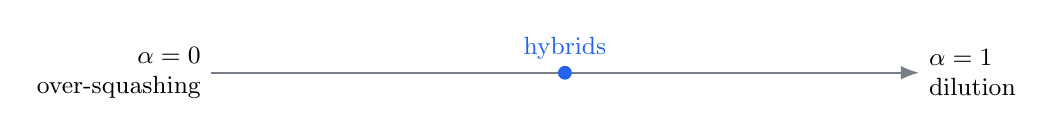
\begin{tikzpicture}
    \draw[-{Latex},thick,ink!60] (0,0) -- (9,0);
    \node[left,font=\small,align=right] at (0,0) {$\alpha=0$\\over-squashing};
    \node[right,font=\small,align=left] at (9,0) {$\alpha=1$\\dilution};
    \node[above,font=\small,accent] at (4.5,0.05) {hybrids};
    \fill[accent] (4.5,0) circle (2.5pt);
  \end{tikzpicture}
\end{frame}

\begin{frame}{Research question and hypotheses}
  \textbf{Question.} Do graph structure (effective resistance) and task range predict where on the local-to-global spectrum (best $\alpha$) a model should sit? Can mechanistic measures explain why?
  \vspace{0.6em}
  \begin{description}[H4]
    \item[H1] At $\alpha=0$, Jacobian sensitivity decays with $R(u,v)$ (negative log-log slope) more steeply than for the transformer; hybrids in between
    \item[H2] Normalised attention entropy rises with graph size for attention models
    \item[H3] Peptides-func is short-range (Bamberger et al. 2025), so expect a low best $\alpha$
    \item[H4] Best $\alpha$ increases with effective resistance and with task range
  \end{description}
  \vspace{0.4em}
  \snote{Deliverable: a phase diagram. x = effective resistance, y = task range, colour = best $\alpha$. The transformer's Jacobian slope serves as a size-confound baseline.}
\end{frame}

\begin{frame}{Gates: checks before any claim}
  \centering
  \small
  \begin{tabular}{@{}lL{0.62\textwidth}l@{}}
    \toprule
    Gate & Criterion & Status \\
    \midrule
    \textbf{G0} & Rebuilt 4-layer hybrid, $\alpha=0.5$, seed 0: test AP $\ge 0.652$ on Peptides-func. $\alpha=0$ and $\alpha=1$ must also train & pending (Colab) \\
    \addlinespace
    \textbf{G1} & Training is sound: mean test AP $\alpha=0.5 \ge 0.63$, $\alpha=1 \ge 0.60$, GCN $\ge 0.66$ (or the gap documented) & pending \\
    \addlinespace
    \textbf{G2} & Measurements are interpretable: Jacobian slope difference vs $\alpha=1$ with a graph-clustered bootstrap CI & pending \\
    \bottomrule
  \end{tabular}
  \vspace{0.8em}

  \raggedright\snote{If G1 fails, change one thing at a time on seed 0: training curves, then lr/warmup, then dropout, then BatchNorm vs LayerNorm, then 300 epochs.}
\end{frame}

% =====================================================================
\section{Datasets}

\begin{frame}{Datasets at a glance}
  \centering
  \footnotesize
  \begin{tabular}{@{}L{0.19\textwidth}L{0.19\textwidth}L{0.18\textwidth}L{0.13\textwidth}L{0.17\textwidth}@{}}
    \toprule
    Dataset & Graphs & Task & Metric & Role \\
    \midrule
    Peptides-func (LRGB) & 15,535 molecules, $\sim$151 nodes & 10-label graph classification & macro AP & main benchmark \\
    Peptides-struct (LRGB) & same graphs & 11-target regression & MAE & task-range axis (planned) \\
    Reddit hyperlinks (SNAP) & 1 graph, 35,776 nodes & node regression & rel.\ MSE per hop band & parallel node track \\
    LamaH-CE rivers & 32 gauge trees, 5--35 nodes & discharge, 1/3/7 days ahead & NRMSE, NSE & real-world tree test \\
    Synthetic trees & 96 trees, 63/127 nodes & near/far query sum & MSE & controlled test \\
    synthetic-tiny & 8--30 nodes & Peptides schema & AP & unit tests, smoke runs \\
    \bottomrule
  \end{tabular}
\end{frame}

\begin{frame}{Peptides-func and Peptides-struct (LRGB)}
  \begin{columns}[T]
    \begin{column}{0.55\textwidth}
      \begin{itemize}
        \item 15,535 graphs; average $\approx$151 nodes, $\approx$307 edges, diameter $\approx$57 \snote{(Dwivedi et al. 2022)}
        \item Split $\approx$70/15/15 (10,873 / 2,331 / 2,331)
        \item Atoms: 9 categorical columns. Bonds: 3 columns. All \emph{embedded}, not passed through Linear
        \item RWSE positional encoding, 20 steps: $\mathrm{pe}_v = [(D^{-1}A)^k_{vv}]_{k=1}^{20}$
      \end{itemize}
    \end{column}
    \begin{column}{0.42\textwidth}
      \begin{itemize}
        \item \textbf{func}: BCE loss, macro AP
        \item \textbf{struct}: L1 loss, MAE (Phase 4)
        \item Same graphs, different task: a test of whether range depends on the task
        \item \alert{Caveat:} the graphs are near-trees, so $R \approx$ hops. ``Resistance beats hops'' cannot be shown here
      \end{itemize}
    \end{column}
  \end{columns}
\end{frame}

\begin{frame}{Reddit, rivers and synthetic trees}
  \begin{columns}[T]
    \begin{column}{0.33\textwidth}
      \textbf{Reddit (SNAP)} \snote{(Kumar et al. 2018)}
      \begin{itemize}\small
        \item Subreddits; 286,561 body hyperlinks, used undirected
        \item 86 averaged post features
        \item \textbf{Distance split} by BFS from an anchor: train 0--1 hops, val 2, test 3+
        \item \textbf{Random control}: same sizes
      \end{itemize}
    \end{column}
    \begin{column}{0.33\textwidth}
      \textbf{LamaH-CE rivers} \snote{(Klingler et al. 2021)}
      \begin{itemize}\small
        \item Upstream gauge trees, depth 1--8
        \item 27 development and 5 held-out outlets
        \item Inputs: weather, or weather + flow
        \item Splits by time: 1981--99 / 2000--05 / 2006--17
      \end{itemize}
    \end{column}
    \begin{column}{0.33\textwidth}
      \textbf{Synthetic trees (v1)}
      \begin{itemize}\small
        \item $N\in\{63,127\}$, depth $\in\{4,8\}$
        \item Early, uniform or late growth profiles
        \item 4 nodes marked at 1 hop, 4 at 4 hops; the root query picks near or far
        \item Reference MSE: oracle 0, topology-blind 0.5
      \end{itemize}
    \end{column}
  \end{columns}
\end{frame}

% =====================================================================
\section{Replicating over-squashing and attention dilution}

\begin{frame}{What has been verified so far}
  \centering
  \footnotesize
  \begin{tabular}{@{}lll@{}}
    \toprule
    Experiment & Purpose & Status \\
    \midrule
    R1 Pilot LRGB replication & GCN / GPS vs published numbers & done \pilot, 1 seed \\
    R2 Pilot mechanistic notebook & Jacobian vs $R$, entropy vs size & done, \alert{flawed setup} \\
    R3 Pilot Reddit & virtual node helps far nodes & done \pilot, unfair baseline \\
    Unit tests & analytic sanity of all measures & \textcolor{good}{125 passed (CPU)} \\
    Demos 1--3 & mechanisms on real model code & \illus \\
    Synthetic tree sweep v1 & MP vs hybrid vs attention & done, confounded \\
    \midrule
    G0 / Phase 2 sweep / real Reddit & re-baseline and measure & \alert{not run} \\
    \bottomrule
  \end{tabular}
\end{frame}

\begin{frame}{Pilot LRGB replication on Peptides-func \pilot}
  \begin{columns}[c]
    \begin{column}{0.5\textwidth}
      \centering
      \begin{tabular}{@{}lccc@{}}
        \toprule
        Model & Val AP & Test AP & Published \\
        \midrule
        GPS & 0.6702 & \textbf{0.6518} & 0.6535 \\
        GCN & 0.6545 & \textbf{0.6263} & $\approx$0.686 \\
        \bottomrule
      \end{tabular}
    \end{column}
    \begin{column}{0.46\textwidth}
      \begin{itemize}
        \item RWSE, 4 layers, hidden 96, 1 seed
        \item \textcolor{good}{GPS reproduces} the published value
        \item GCN is 0.06 short of Tönshoff et al.'s tuned value, so this is only a \alert{partial} replication
        \item G0's 0.652 threshold comes from this GPS run
      \end{itemize}
    \end{column}
  \end{columns}
\end{frame}

\begin{frame}{Pilot mechanistic notebook \pilot}
  \begin{columns}[T]
    \begin{column}{0.5\textwidth}
      \textbf{Jacobian vs resistance} (log-log slope, 240 pairs)
      \begin{center}\small
      \begin{tabular}{@{}lccc@{}}
        \toprule
        & GINE & Transf. & GPS \\
        \midrule
        slope & $-1.76$ & $-0.48$ & $-0.81$ \\
        $r$ & $-0.78$ & $-0.41$ & $-0.69$ \\
        test AP & 0.54 & 0.27 & 0.24 \\
        \bottomrule
      \end{tabular}
      \end{center}
      \textbf{Entropy vs size} (400 graphs)
      \begin{itemize}\small
        \item Raw $H$ rises for both models ($r=+0.88$, $+0.91$)
        \item $H/\log N$ rises \emph{only for GPS} ($r=+0.60$), not for the transformer ($r=-0.09$)
      \end{itemize}
    \end{column}
    \begin{column}{0.46\textwidth}
      \begin{alertblock}{Caveats: not citable as results}
        \small
        \begin{itemize}
          \item 30 epochs, 1 seed; the attention models did not train
          \item Atom codes passed through \texttt{nn.Linear}; no positional encoding
          \item Entropy computed on head-averaged attention
          \item Shared LayerNorm; sum pooling
        \end{itemize}
        Nine bugs were fixed in Phase 1 (\texttt{gnn\_mech})
      \end{alertblock}
    \end{column}
  \end{columns}
\end{frame}

\begin{frame}{Pilot Reddit: virtual node vs SAGE by hop band \pilot}
  \begin{columns}[c]
    \begin{column}{0.52\textwidth}
      \centering\small
      \begin{tabular}{@{}rrrrr@{}}
        \toprule
        Hop & $n$ & SAGE & VMN & Cut \\
        \midrule
        1 & 1,454 & 16,808 & 14,808 & 12\% \\
        2 & 17,876 & 90,056 & 56,115 & 38\% \\
        3 & 7,269 & 194,509 & 95,359 & 51\% \\
        4 & 613 & 207,113 & 77,806 & 62\% \\
        $\ge$5 & 57 & 326,334 & 62,993 & 81\% \\
        \bottomrule
      \end{tabular}

      \snote{Mean test MSE over 100 seeds (raw units)}
    \end{column}
    \begin{column}{0.44\textwidth}
      \begin{itemize}
        \item The gain from a global shortcut grows with distance
        \item \alert{Caveats}
          \begin{itemize}\small
            \item Only VMN had an input projection (unfair baseline)
            \item The target (character count) is almost a function of the node's own features
            \item The distance split confounds ``far'' with ``out of distribution''
          \end{itemize}
        \item Phase 2 fixes all three
      \end{itemize}
    \end{column}
  \end{columns}
\end{frame}

\begin{frame}{Demo 1: Jacobian decays with hops \illus}
  \centering
  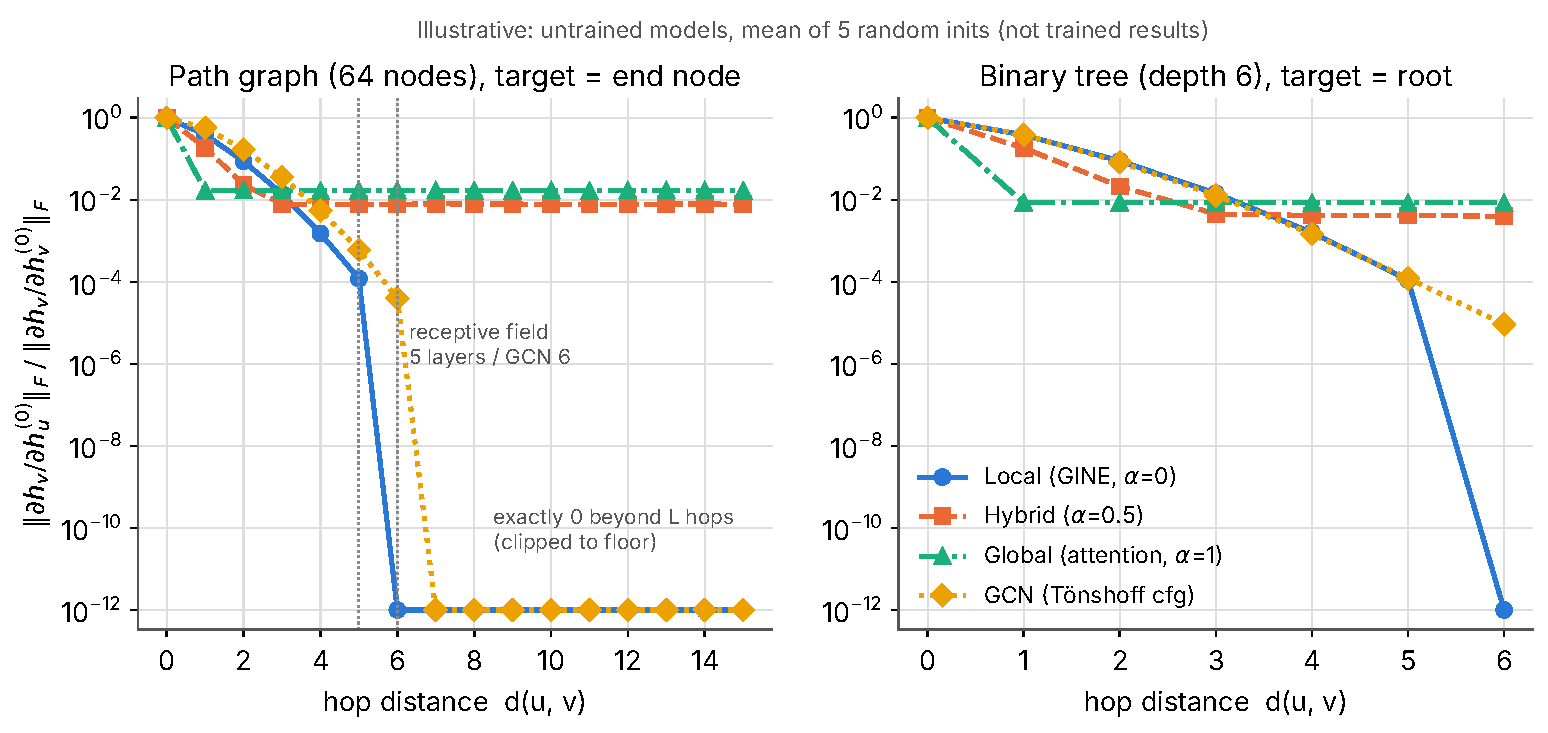
\includegraphics[width=0.86\textwidth]{demo_jacobian_vs_hops_untrained.pdf}

  \small
  MP loses $\approx$3--10$\times$ per hop and is exactly 0 beyond $L$ hops. Attention is flat at $\approx 1/N$. The $\alpha=0.5$ hybrid follows the local curve for 2--3 hops, then settles on a floor half as high.
\end{frame}

\begin{frame}{Demo 2: attention dilution with graph size \illus}
  \centering
  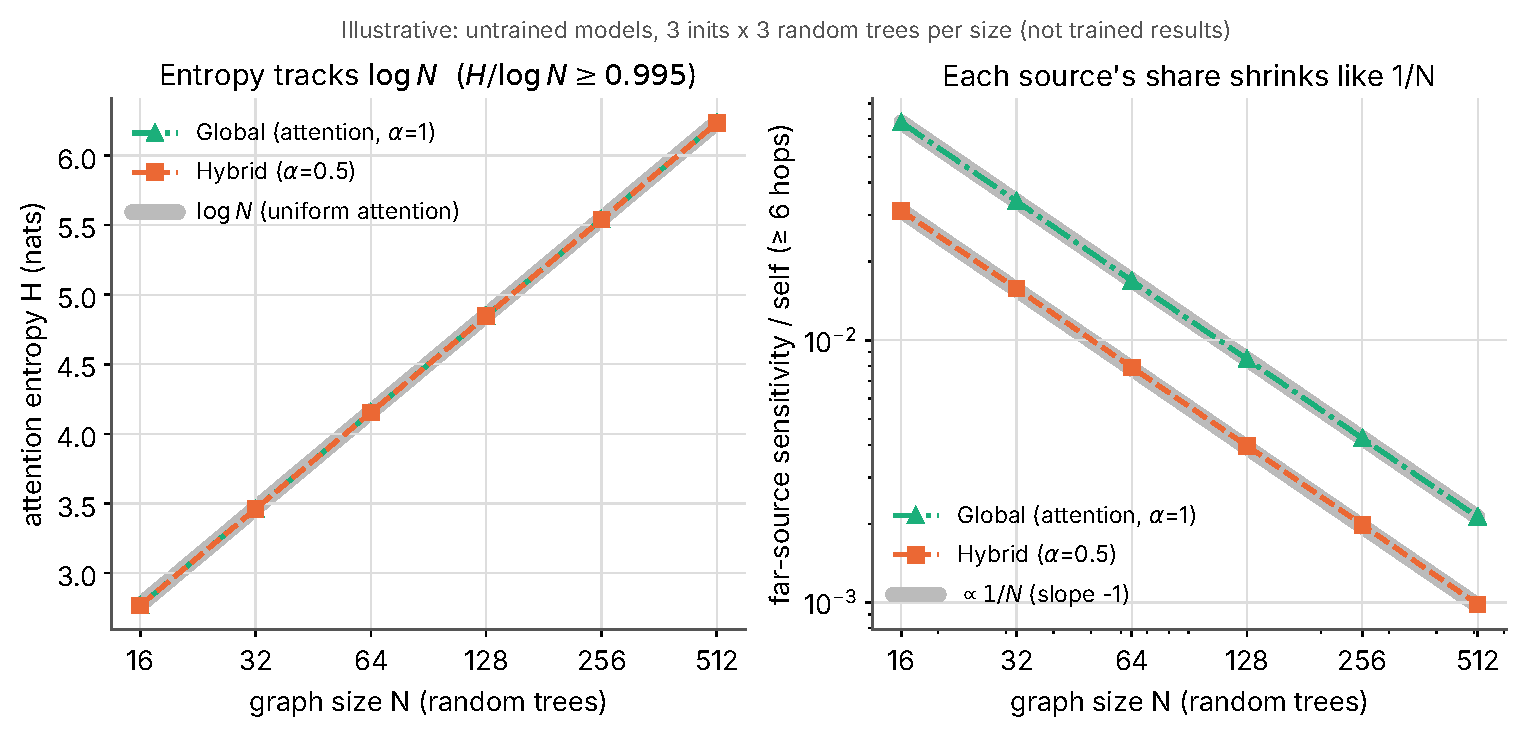
\includegraphics[width=0.84\textwidth]{demo_attention_dilution_untrained.pdf}

  \small
  Entropy lies on $\log N$ ($H/\log N \ge 0.995$). Sensitivity to sources $\ge$6 hops away falls exactly as $1/N$, e.g.\ global: $6.8\times10^{-2}$ at $N=16$ and $2.1\times10^{-3}$ at $N=512$.
\end{frame}

\begin{frame}{Demo 3: range-measure sanity on a 150-node path \illus}
  \centering\small
  \begin{tabular}{@{}lcc@{}}
    \toprule
    Model (untrained) & Node-level range, hops (mean / max) & Graph-level Hessian range \\
    \midrule
    Local $\alpha=0$ (5 layers) & 0.67 / 0.69 \;($\le 5$ \textcolor{good}{\checkmark}) & undefined (ReLU-only) \\
    Hybrid $\alpha=0.5$ & 18.7 / 25.8 & not run \\
    Global $\alpha=1$ & 34.3 / 47.0 & not run \\
    GCN (6 layers, GELU) & 0.89 / 0.89 & \alert{17.7} \\
    \bottomrule
  \end{tabular}
  \vspace{0.8em}
  \raggedright
  \begin{itemize}
    \item The node-level range respects the receptive field and grows once attention is mixed in
    \item The Hessian range reaches $\approx$18 hops, far past GCN's 6-hop reach: mean pooling plus a nonlinear head couples all pairs
    \item[$\Rightarrow$] Models are compared using the \textbf{node-level} range
  \end{itemize}
\end{frame}

\begin{frame}{Synthetic tree sweep v1: MP fails the 4-hop query}
  \begin{columns}[c]
    \begin{column}{0.5\textwidth}
      \centering\small
      \begin{tabular}{@{}lccc@{}}
        \toprule
        Model & Near & Far & Balanced \\
        \midrule
        MP ($\alpha=0$) & 0.0036 & \alert{1.0094} & 0.5065 \\
        $\alpha=0.25$ & \textbf{0.0024} & 0.0129 & \textbf{0.0077} \\
        $\alpha=0.50$ & 0.0074 & 0.0147 & 0.0110 \\
        $\alpha=0.75$ & 0.0050 & \textbf{0.0122} & 0.0086 \\
        Attn ($\alpha=1$) & 0.0093 & 0.0189 & 0.0141 \\
        \bottomrule
      \end{tabular}

      \snote{Test MSE; predicting zero gives 1. 21 fits, about 49 min.}
    \end{column}
    \begin{column}{0.46\textwidth}
      \begin{itemize}
        \item MP solves the 1-hop query but fails the 4-hop one, though 4 hops lie inside its 8-layer reach
        \item Every hybrid beats pure attention
        \item \alert{Confounded}: different target draws, mean aggregation for a sum target, attention-only hop bias, LayerNorm, unequal parameter counts
        \item Not re-verified here (archive missing)
      \end{itemize}
    \end{column}
  \end{columns}
\end{frame}

% =====================================================================
\section{The pipeline and models}

\begin{frame}{End-to-end pipeline (\texttt{gnn\_mech})}
  \centering
  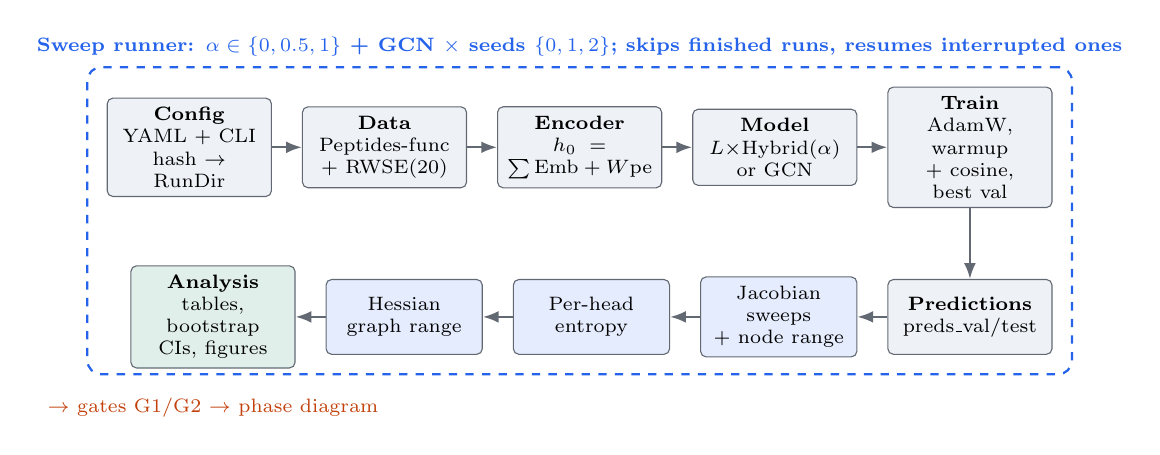
\begin{tikzpicture}[
      box/.style={draw=ink!70,fill=soft,rounded corners=2pt,font=\scriptsize,align=center,minimum height=0.95cm,text width=1.85cm},
      mbox/.style={box,fill=accent!12,text width=1.75cm},
      arr/.style={-{Latex[length=2mm]},thick,ink!70},
      node distance=0.38cm]
    \node[box] (cfg) {\textbf{Config}\\YAML + CLI\\hash $\to$ RunDir};
    \node[box,right=of cfg] (data) {\textbf{Data}\\Peptides-func\\+ RWSE(20)};
    \node[box,right=of data] (enc) {\textbf{Encoder}\\$h_0=\sum\mathrm{Emb}+W\mathrm{pe}$};
    \node[box,right=of enc] (model) {\textbf{Model}\\$L\times$Hybrid($\alpha$)\\or GCN};
    \node[box,right=of model] (train) {\textbf{Train}\\AdamW, warmup\\+ cosine, best val};
    \node[box,below=0.9cm of train] (pred) {\textbf{Predictions}\\preds\_val/test};
    \node[mbox,left=of pred] (jac) {Jacobian sweeps\\+ node range};
    \node[mbox,left=of jac] (ent) {Per-head\\entropy};
    \node[mbox,left=of ent] (hes) {Hessian\\graph range};
    \node[box,left=of hes,fill=good!12] (ana) {\textbf{Analysis}\\tables, bootstrap\\CIs, figures};
    \draw[arr] (cfg) -- (data); \draw[arr] (data) -- (enc); \draw[arr] (enc) -- (model); \draw[arr] (model) -- (train);
    \draw[arr] (train) -- (pred);
    \draw[arr] (pred) -- (jac); \draw[arr] (jac) -- (ent); \draw[arr] (ent) -- (hes); \draw[arr] (hes) -- (ana);
    \begin{scope}[on background layer]
      \node[draw=accent,dashed,thick,rounded corners=5pt,fit=(cfg)(train)(pred)(hes),inner sep=7pt,
            label={[font=\scriptsize\bfseries,accent]above:Sweep runner: $\alpha\in\{0,0.5,1\}$ + GCN $\times$ seeds $\{0,1,2\}$; skips finished runs, resumes interrupted ones}] (sweep) {};
    \end{scope}
    \node[below=0.25cm of ana,font=\scriptsize,warm] {$\to$ gates G1/G2 $\to$ phase diagram};
  \end{tikzpicture}
  \vspace{0.3em}

  \snote{Outputs per run: \texttt{metrics.json}, \texttt{measurements.json}, \texttt{best.pt}, \texttt{history.json}. All measures run on the best-validation checkpoint in eval mode.}
\end{frame}

\begin{frame}{HybridLayer, exactly as implemented}
  \small
  \begin{align*}
    h_{\text{loc}} &= \mathrm{BN}_{\text{loc}}\big(\mathrm{GINE}(x, E, e)\big), \qquad
    h_{\text{glb}} = \mathrm{BN}_{\text{glb}}\big(\mathrm{MHA}(x)\big) \\
    x' &= x + \mathrm{Dropout}\big((1-\alpha)\,h_{\text{loc}} + \alpha\,h_{\text{glb}}\big) \\
    x'' &= \mathrm{BN}_{\text{ffn}}\big(x' + \mathrm{FFN}(x')\big), \qquad \mathrm{FFN} = \mathrm{Lin}(d\!\to\!2d)\,\text{ReLU}\,\text{Dropout}\,\mathrm{Lin}(2d\!\to\!d)
  \end{align*}
  \begin{columns}[T]
    \begin{column}{0.5\textwidth}
      \textbf{GINE branch}
      \[ \mathrm{GINE}(x)_v = \mathrm{MLP}\Big((1+\epsilon)x_v + \!\!\!\sum_{u\in\mathcal N(v)}\!\!\!\mathrm{ReLU}(x_u + e_{uv})\Big) \]
      \snote{Learnable $\epsilon$; edge embeddings already have width $d$}
    \end{column}
    \begin{column}{0.46\textwidth}
      \textbf{MHA branch}
      \begin{itemize}\small
        \item Dense attention \emph{within} each graph, with a padding mask
        \item 4 heads, $\mathrm{softmax}(QK^\top/\sqrt{d_h})V$, attention dropout 0.1
        \item $\alpha=0$: MHA not built; $\alpha=1$: GINE not built
      \end{itemize}
    \end{column}
  \end{columns}
  \snote{Model: InputEncoder $\to L\times$ HybridLayer $\to$ mean pool $\to$ MLP head $\to$ 10 logits. All norms are BatchNorm, as in GraphGPS.}
\end{frame}

\begin{frame}{Baselines: GCN (Tönshoff-aligned) and the Reddit models}
  \begin{columns}[T]
    \begin{column}{0.5\textwidth}
      \textbf{GCN} \snote{(Tönshoff et al. 2023)}
      \[ x \leftarrow x + \mathrm{Dropout}\big(\mathrm{GELU}(\tilde D^{-1/2}\tilde A\tilde D^{-1/2} x W)\big) \]
      \begin{itemize}\small
        \item 6 layers, hidden 235, no per-layer norm, 3-layer head
        \item 250 epochs, batch 200, RWSE 20; ignores edge features
        \item Target $\approx$0.686 AP; remaining difference: how RWSE is injected
      \end{itemize}
    \end{column}
    \begin{column}{0.46\textwidth}
      \textbf{Reddit node regression}
      \begin{itemize}\small
        \item \textbf{SAGE}: Linear(in$\to$64) $\to$ 3$\times$SAGEConv
          \[ h_v' = W_1 h_v + W_2\,\mathrm{mean}_{u\in\mathcal N(v)} h_u \]
        \item \textbf{VMN}: the same network plus one master node linked to every node, so all pairs are within 2 hops
        \item VMN is the node-task analogue of $\alpha\to1$
        \item Fix: both models now have the input projection; 30 seeds each
      \end{itemize}
    \end{column}
  \end{columns}
\end{frame}

\begin{frame}{Model sizes and the $\alpha$ grid}
  \begin{columns}[c]
    \begin{column}{0.6\textwidth}
      \centering\footnotesize
      \begin{tabular}{@{}lcccr@{}}
        \toprule
        Config & hidden & $L$ & heads & params \\
        \midrule
        Hybrid $\alpha=0$ (GINE) & 96 & 5 & 4 & 311,055 \\
        Hybrid $\alpha=0.5$ (GPS-like) & 96 & 5 & 4 & 498,255 \\
        Hybrid $\alpha=1$ (transformer) & 96 & 5 & 4 & 404,170 \\
        GCN (Tönshoff) & 235 & 6 & -- & 491,865 \\
        G0 pilot-equivalence $\alpha=0.5$ & 96 & 4 & 4 & 404,654 \\
        \bottomrule
      \end{tabular}

      \snote{LRGB budget is 500k. Training: 200 epochs, batch 128, AdamW lr $10^{-3}$, 5 warmup epochs.}
    \end{column}
    \begin{column}{0.36\textwidth}
      \begin{itemize}
        \item \textbf{Phase 2}: $\alpha\in\{0, 0.5, 1\}$ + GCN, 3 seeds (12 runs)
        \item \textbf{Phase 3}: $\alpha\in\{0, .25, .5, .75, 1\}$, 3 seeds
        \item \textbf{Rivers}: $\alpha\in\{0, .25, .5, .75, 1\}$
        \item \alert{Confound}: parameter count changes with $\alpha$ because unused branches are not built
      \end{itemize}
    \end{column}
  \end{columns}
\end{frame}

% =====================================================================
\section{Measures}

\begin{frame}{Effective resistance and Jacobian sensitivity}
  \begin{columns}[T]
    \begin{column}{0.47\textwidth}
      \textbf{Effective resistance}
      \[ R(u,v) = (e_u - e_v)^\top L^+ (e_u - e_v) \]
      \begin{itemize}\small
        \item $L = D - A$; $L^+ = (L + \tfrac1n J)^{-1}$ on the largest connected component
        \item Graph level: mean of $R$ over all pairs
        \item Tests: path $\Rightarrow R=$ hops; complete graph $\Rightarrow R=2/n$
      \end{itemize}
    \end{column}
    \begin{column}{0.5\textwidth}
      \textbf{Jacobian sensitivity}
      \[ J(u,v) = \Big\|\frac{\partial h_v^{(L)}}{\partial h_u^{(0)}}\Big\|_F \]
      \begin{itemize}\small
        \item Taken w.r.t.\ the embedded input $h_0$
        \item 200 graphs $\times$ 4 targets $\times$ 32 sources, stratified by $R$
        \item Slope $b$: $\log_{10} J = a + b\log_{10} R$ (also vs hops; size-controlled with $+\beta_N\log_{10} n$)
        \item G2: $\Delta b = b_\alpha - b_{\alpha=1}$, \textbf{graph-clustered bootstrap} (resample graphs, 1000 reps)
        \item One batched backward per target: $\approx$30$\times$ speedup
      \end{itemize}
    \end{column}
  \end{columns}
\end{frame}

\begin{frame}{Per-head attention entropy (dilution)}
  For layer $\ell$, head $h$, graph with $N$ nodes and attention $a_{ij}$:
  \[ H_{\ell,h} = \frac1N\sum_{i=1}^{N}\Big(-\sum_{j=1}^{N} a^{(\ell,h)}_{ij}\log a^{(\ell,h)}_{ij}\Big),\qquad
     \tilde H_{\ell,h} = \frac{H_{\ell,h}}{\log N}\in[0,1] \]
  \begin{itemize}
    \item Computed \textbf{per head}; averaging heads first inflates entropy (a pilot bug)
    \item Uniform attention $\Rightarrow \tilde H = 1$ (unit-tested)
    \item 500 graphs: Pearson $r(N, H)$, $r(N, \tilde H)$, per-layer means, graph-bootstrap CIs
    \item Undefined for $\alpha=0$
  \end{itemize}
  \begin{block}{$\alpha$ as the interpolation knob}
    \small $\alpha=0$: receptive field of $L$ hops (over-squashing regime). $\alpha>0$: every pair connected in one layer (dilution regime).
    Jacobian slope, entropy, range and AP are all reported \emph{as functions of $\alpha$}; best $\alpha$ per resistance bin $\to$ phase diagram.
  \end{block}
\end{frame}

\begin{frame}{Range measure (Bamberger et al., ICML 2025)}
  \begin{columns}[T]
    \begin{column}{0.54\textwidth}
      \small
      Implemented following Gutteridge's \texttt{range-measure} repository.
      \begin{align*}
        \text{node: } I_{vu} &= \textstyle\sum_{k,d}\big|\partial y_{v,k}/\partial x_{u,d}\big| \\
        \text{graph: } I_{uw} &= \textstyle\sum_{k,d,d'}\big|\partial^2 y_k/\partial x_{u,d}\,\partial x_{w,d'}\big| \\
        \rho_v &= \frac{\sum_u I_{vu}\, d(v,u)}{\sum_u I_{vu}}, \quad d\in\{\text{hops}, R\}
      \end{align*}
      Graph range is the mean over nodes; dataset range is the mean over graphs.
    \end{column}
    \begin{column}{0.42\textwidth}
      \begin{itemize}\small
        \item \textbf{Node-level} (Jacobian): reuses the Jacobian sweeps; matches the paper's LRGB setting
        \item \textbf{Graph-level} (Hessian): 30 graphs, $\approx$50\,s per graph on CPU
        \item \alert{Caveats}: the Hessian is zero for ReLU-only $\alpha=0$; pooling into a nonlinear head extends the range past the receptive field
        \item Reading rule: all hop ranges $\le L/2 \Rightarrow$ short-range
      \end{itemize}
    \end{column}
  \end{columns}
\end{frame}


% =====================================================================
\section{Results}

\begin{frame}{River experiment: setup}
  \begin{columns}[c]
    \begin{column}{0.44\textwidth}
      \begin{itemize}\small
        \item GRU temporal encoder (90 days) $\to$ 8 spatial layers, width 64, 4 heads
        \item Each layer: $(1-\alpha)\,\mathrm{LN(MP)} + \alpha\,\mathrm{LN(Attn)}$
        \item MP: upstream$\to$downstream, mean aggregation
        \item Attention over ancestors, with a hop bias
        \item Baselines: outlet-only GRU, upstream pooling, persistence
        \item 72 fits, 3 seeds, $\approx$28.5 GPU-h
        \item Hypothesis: faster upstream growth $V(r)$ means a larger gain over MP
      \end{itemize}
    \end{column}
    \begin{column}{0.54\textwidth}
      \centering
      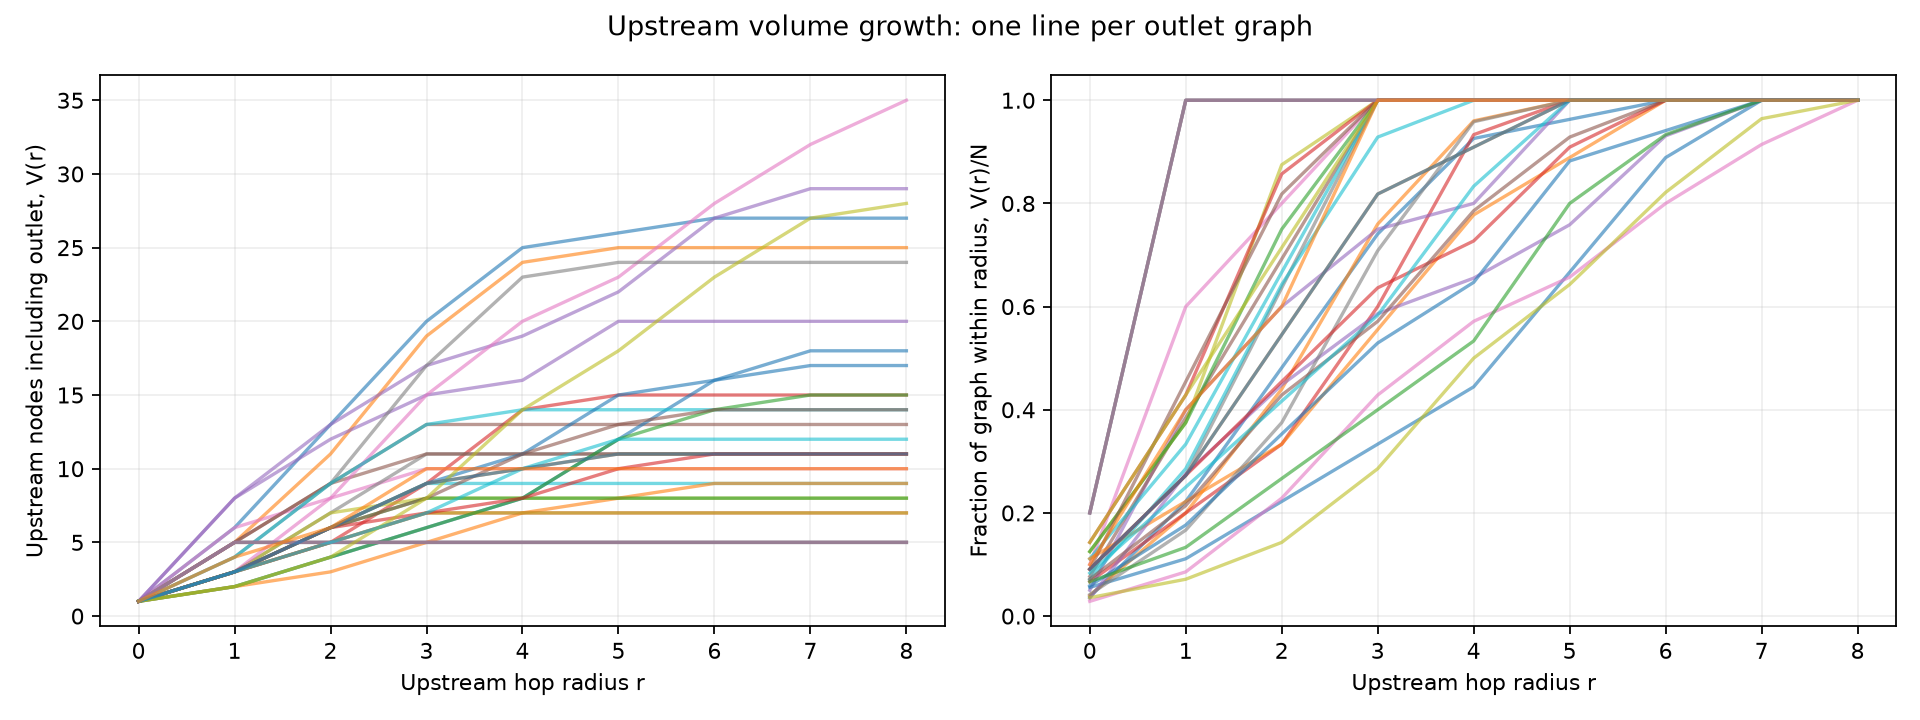
\includegraphics[width=\textwidth]{river_upstream_growth_profiles.png}

      \snote{$V(r)$: upstream nodes within $r$ hops. It saturates at $N$.}
    \end{column}
  \end{columns}
\end{frame}

\begin{frame}{Held-out results: the $\alpha$ curve (test NRMSE, lower is better)}
  \begin{columns}[c]
    \begin{column}{0.46\textwidth}
      \centering\small
      \begin{tabular}{@{}lcc@{}}
        \toprule
        Model & Weather & Weather+flow \\
        \midrule
        MP ($\alpha=0$) & 0.2666 & 0.1691 \\
        $\alpha=0.25$ & 0.2628 & 0.1722 \\
        $\alpha=0.5$ & 0.2489 & 0.1706 \\
        $\alpha=0.75$ & \textbf{0.2409} & 0.1716 \\
        Attention ($\alpha=1$) & 0.2426 & 0.1713 \\
        Upstream pooling & 0.2437 & \textbf{0.1689} \\
        Outlet-only GRU & 0.2600 & 0.1696 \\
        \bottomrule
      \end{tabular}
    \end{column}
    \begin{column}{0.5\textwidth}
      \begin{itemize}\small
        \item \textbf{Weather only}: $\alpha=0.75$ is best, \textcolor{good}{9.6\% better than MP}
        \item But only 0.7\% better than attention and 1.1\% better than pooling, so the gain comes mostly from \emph{global access}
        \item \textbf{Weather+flow}: \alert{no gain}; every $\alpha>0$ is slightly worse than MP and pooling is best
        \item Validation-chosen $\alpha$ is unstable once flow is given
        \item Mean NSE in the weather regime is negative ($-0.30$ at $\alpha=0.75$)
      \end{itemize}
    \end{column}
  \end{columns}
\end{frame}

\begin{frame}{$\alpha$ curves per held-out outlet}
  \centering
  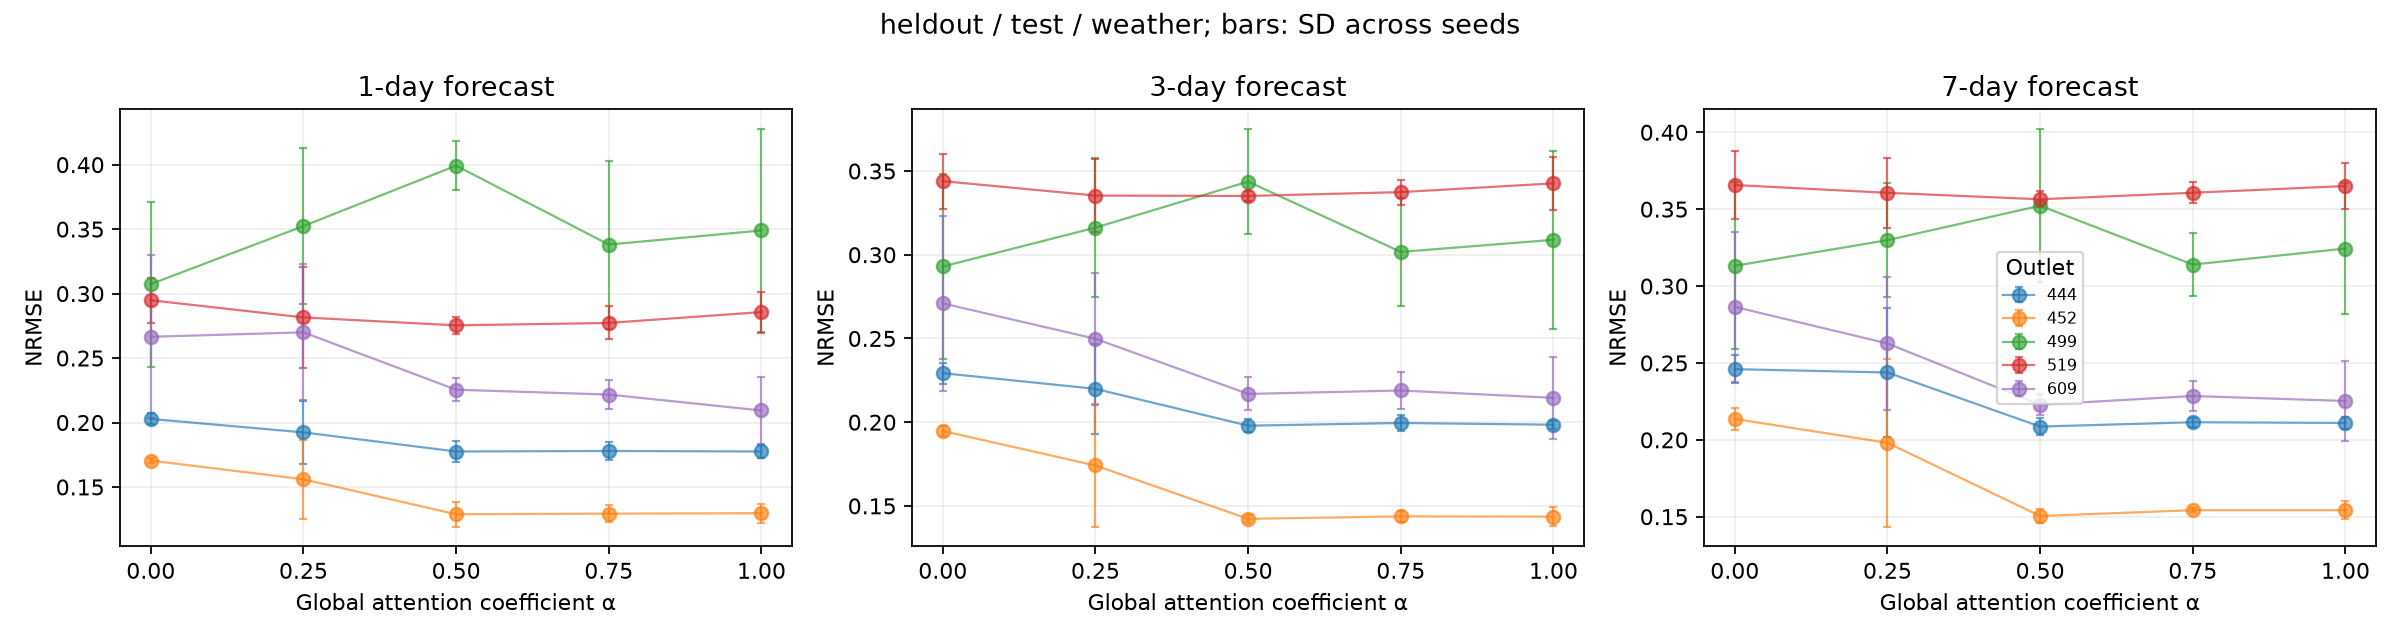
\includegraphics[width=0.8\textwidth]{river_alpha_curves_heldout_weather.png}\\[-0.2em]
  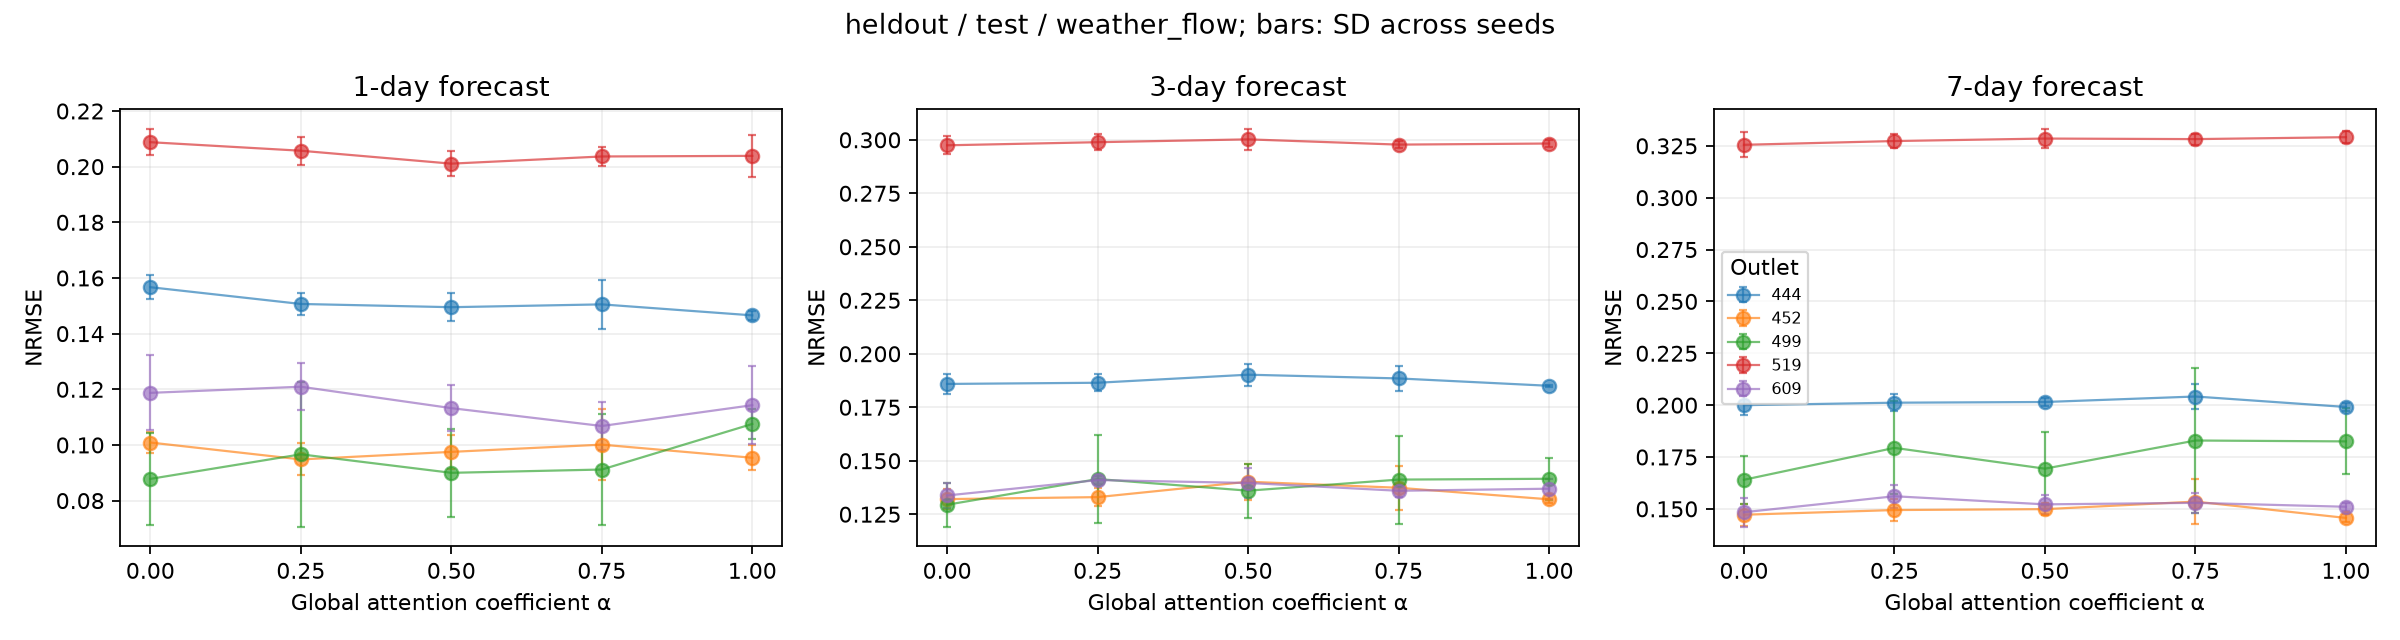
\includegraphics[width=0.8\textwidth]{river_alpha_curves_heldout_weather_flow.png}

  \snote{Top: weather (most outlets improve up to $\alpha\ge0.5$; the largest graph, 499, does not). Bottom: weather+flow (flat).}
\end{frame}

\begin{frame}{Context ablation: a hint of over-squashing}
  \begin{columns}[c]
    \begin{column}{0.52\textwidth}
      \centering\small
      \begin{tabular}{@{}lccc@{}}
        \toprule
        Weather & Full & Radius 2 & Radius 0 \\
        \midrule
        MP ($\alpha=0$) & 0.2666 & 0.2673 & \textbf{0.2584} \\
        $\alpha=0.75$ & \textbf{0.2409} & 0.2695 & 0.2741 \\
        Attention & \textbf{0.2426} & 0.2583 & 0.2791 \\
        \bottomrule
      \end{tabular}

      \snote{Held-out test NRMSE, mean over horizons. Radius $r$: dynamic inputs kept only within $r$ hops.}
    \end{column}
    \begin{column}{0.44\textwidth}
      \begin{itemize}\small
        \item MP does \emph{better} when upstream inputs are hidden (same on the development set)
        \item Attention and the hybrid exploit upstream context: about $-12\%$ NRMSE vs radius 0
        \item \alert{Consistent with} over-squashing, but also with optimisation, mean-aggregation or parameter effects
        \item The ablation masks inputs; it does not rewire the graph
      \end{itemize}
    \end{column}
  \end{columns}
\end{frame}

\begin{frame}{Growth $\to$ gain hypothesis: \alert{not supported}}
  \centering
  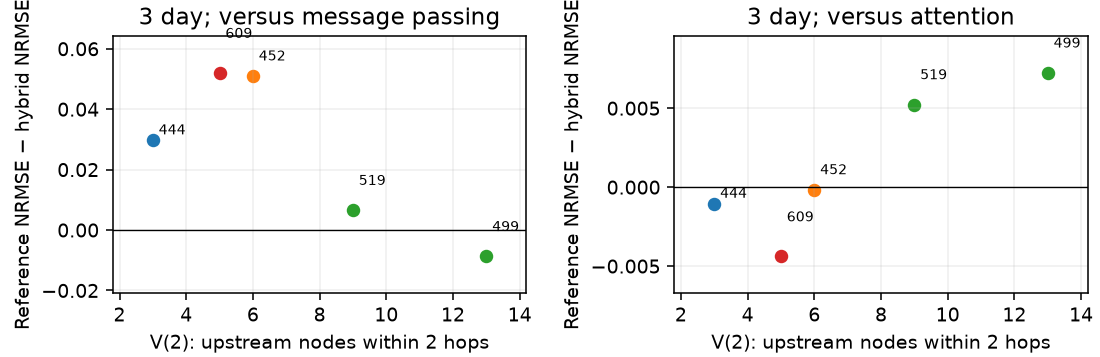
\includegraphics[width=0.6\textwidth]{river_growth_vs_gain_heldout_weather_a075_3day_mp_vs_attn.png}\\[-0.3em]
  {\tiny Held-out, weather, $\alpha=0.75$, 3-day horizon. Positive = hybrid better than the reference.}
  \vspace{0.2em}
  \begin{columns}[T]
    \begin{column}{0.4\textwidth}
      \centering\scriptsize
      \begin{tabular}{@{}rrrr@{}}
        \toprule
        Outlet & Nodes & $V(2)$ & Gain vs MP \\
        \midrule
        444 & 9 & 3 & $+13.1\%$ \\
        609 & 7 & 5 & $+18.8\%$ \\
        452 & 8 & 6 & $+26.2\%$ \\
        519 & 11 & 9 & $+2.9\%$ \\
        499 & 29 & 13 & \alert{$-4.4\%$} \\
        \bottomrule
      \end{tabular}
    \end{column}
    \begin{column}{0.56\textwidth}
      \begin{itemize}\scriptsize
        \item The fastest-growing outlet (499) gains \emph{least}
        \item Spearman $\rho(V(2),\text{gain})$ is $\approx-0.7$ vs MP but $+0.9$ vs attention: \textbf{the sign flips with the reference}
        \item $n=5$; leave-one-group-out ranges span both signs
        \item Development set: after adjusting for size, depth and area, $\rho\approx0$
        \item A graph-conditioned $\alpha$ selector is 2.3\% \emph{worse} than a fixed $\alpha$
      \end{itemize}
    \end{column}
  \end{columns}
\end{frame}

\begin{frame}{Cost vs $\alpha$}
  \begin{columns}[c]
    \begin{column}{0.58\textwidth}
      \centering
      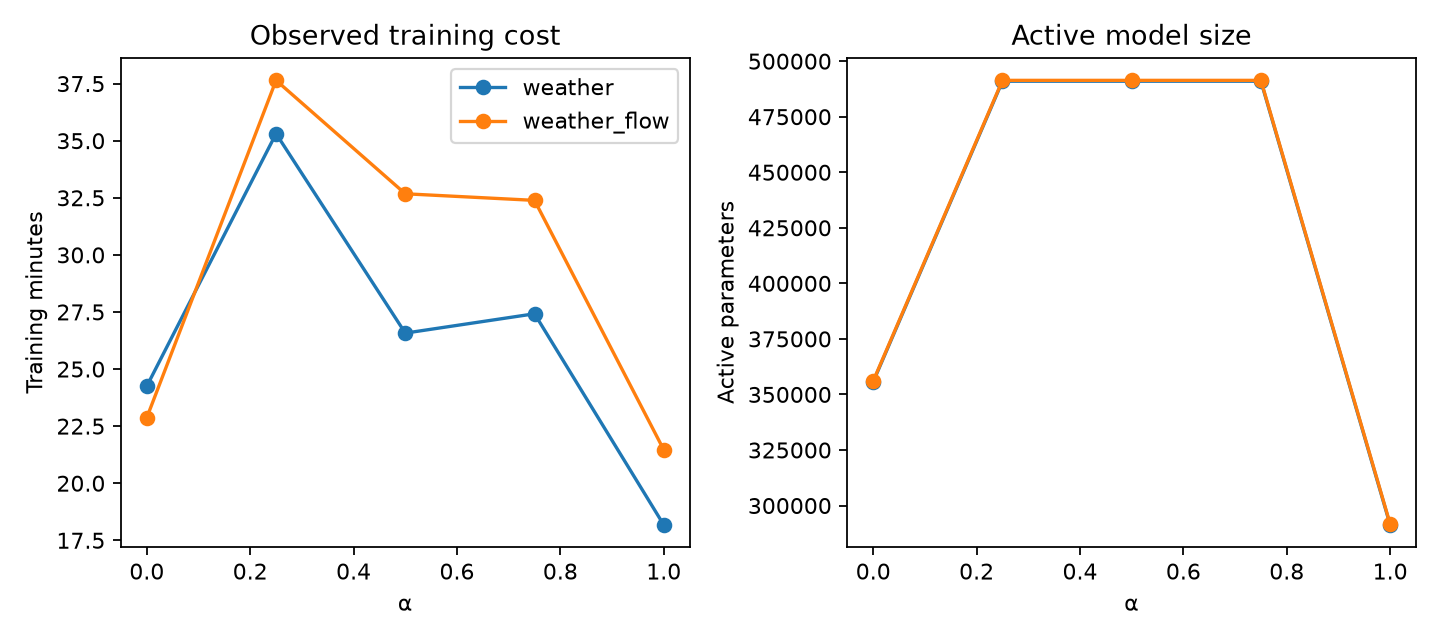
\includegraphics[width=\textwidth]{river_cost_vs_alpha.png}
    \end{column}
    \begin{column}{0.4\textwidth}
      \centering\scriptsize
      \begin{tabular}{@{}lrr@{}}
        \toprule
        Model & Params & s/epoch \\
        \midrule
        MP & 355,715 & 55 \\
        Hybrid & 490,979 & 80--82 \\
        Attention & 291,299 & 55 \\
        Pooling & 26,627 & 15 \\
        Outlet GRU & 22,403 & 11 \\
        \bottomrule
      \end{tabular}
      \begin{itemize}\small
        \item A hybrid takes $\approx1.5\times$ the time per epoch of either endpoint
        \item Pooling matches the best hybrid with $\approx5\%$ of the parameters
      \end{itemize}
    \end{column}
  \end{columns}
\end{frame}

\begin{frame}{Status: what does \emph{not} exist yet}
  \begin{alertblock}{No Phase 2 real-data GPU results yet}
    \begin{itemize}
      \item G0 not run, so the rebuilt hybrid has not been checked against 0.652 AP
      \item Phase 2 sweep (12 runs) not run: no re-baselined AP, no G1/G2, no Jacobian slope CIs, no entropy-vs-size on correctly built models, no range on real Peptides
      \item Aligned Tönshoff GCN not run; only the pilot's 0.6263 exists
      \item Reddit not run on the real graph (SNAP is blocked in the sandbox)
    \end{itemize}
  \end{alertblock}
  \begin{exampleblock}{What is solid}
    Code for Phases 1 and 2 is built and CPU-tested (125 tests pass). Demos confirm the measures behave as theory predicts. River and tree results are real, but small or confounded.
  \end{exampleblock}
\end{frame}

% =====================================================================
\section{Future work}

\begin{frame}{Next: run on Colab (in order)}
  \begin{enumerate}
    \item \textbf{G0}: \texttt{pilot\_equivalence.yaml}, $\alpha=0.5$ needs $\ge0.652$ AP; $\alpha=0$ and $\alpha=1$ must train
    \item \textbf{Phase 2 sweep}: 12 runs, $\approx$5 GPU-h ($\approx$4\,h training + $\approx$1\,h measuring)
    \item \textbf{Range sanity} on real Peptides: $\alpha=0$ mean node range $\le 5$ hops
    \item \textbf{Real Reddit}: reproduce the pilot's band ordering, select a target from the data, then 30 seeds $\times$ \{SAGE, VMN\} $\times$ \{distance, random\}
    \item \textbf{Analysis notebook} $\to$ check G1/G2 $\to$ \texttt{docs/results/phase2.md}
  \end{enumerate}
\end{frame}

\begin{frame}{Later phases}
  \begin{columns}[T]
    \begin{column}{0.5\textwidth}
      \begin{description}[P3]\small
        \item[P3] Full $\alpha$ sweep $\{0,.25,.5,.75,1\}\times3$ seeds; best $\alpha$ per resistance bin; gated-attention baseline
        \item[P4] Task-range axis: Peptides-func vs Peptides-struct
        \item[P5] Synthetic suite: controlled resistance and long-range dependence, distractor injection $\to$ \textbf{phase diagram}
        \item[P6] Predictor of best $\alpha$ from structure + range; held-out check
      \end{description}
    \end{column}
    \begin{column}{0.46\textwidth}
      \textbf{Tree experiment v2} (planned, not run)
      \begin{itemize}\small
        \item Residual Sum-MP/Attention: sum aggregation scaled by $1/\sqrt{\Delta}$, no attention-only hop bias, no amplitude-stripping LayerNorm
        \item Addressed retrieval: $K=4$ vs $16$ candidates at 4 hops
        \item Parameter-matched endpoints
        \item A \textbf{dilution intervention} that adds irrelevant nodes
      \end{itemize}
    \end{column}
  \end{columns}
\end{frame}

% =====================================================================
\section*{Summary}

\begin{frame}{Takeaways}
  \begin{itemize}
    \item The \textbf{mechanisms} show up in real model code: MP sensitivity falls by orders of magnitude within $L$ hops, and attention sensitivity falls as $1/N$ \snote{(untrained demos)}
    \item \textbf{Global access helps when the task needs distant information}: synthetic far query, weather-only rivers ($\alpha=0.75$ is 9.6\% better than MP)
    \item When local history is enough (weather+flow), MP or pooling suffices and \alert{the hybrid only adds cost}
    \item \alert{Graph growth does not predict} the hybrid's gain: the sign flips with the reference model
    \item The pilot Peptides evidence is flawed; the rebuilt, tested pipeline is ready for G0 and the Phase 2 sweep
    \item Goal: a phase diagram of best $\alpha$ against effective resistance and task range
  \end{itemize}
\end{frame}

\begin{frame}[allowframebreaks]{References}
  \scriptsize
  \begin{itemize}
    \item U.~Alon, E.~Yahav. On the Bottleneck of Graph Neural Networks and its Practical Implications. \emph{ICLR}, 2021.
    \item J.~Topping, F.~Di Giovanni, B.~P.~Chamberlain, X.~Dong, M.~M.~Bronstein. Understanding Over-Squashing and Bottlenecks on Graphs via Curvature. \emph{ICLR}, 2022.
    \item F.~Di Giovanni, L.~Giusti, F.~Barbero, G.~Luise, P.~Liò, M.~M.~Bronstein. On Over-Squashing in Message Passing Neural Networks: The Impact of Width, Depth, and Topology. \emph{ICML}, 2023.
    \item M.~Black, Z.~Wan, A.~Nayyeri, Y.~Wang. Understanding Oversquashing in GNNs through the Lens of Effective Resistance. \emph{ICML}, 2023.
    \item L.~Rampášek, M.~Galkin, V.~P.~Dwivedi, A.~T.~Luu, G.~Wolf, D.~Beaini. Recipe for a General, Powerful, Scalable Graph Transformer. \emph{NeurIPS}, 2022.
    \item V.~P.~Dwivedi, L.~Rampášek, M.~Galkin, A.~Parviz, G.~Wolf, A.~T.~Luu, D.~Beaini. Long Range Graph Benchmark. \emph{NeurIPS Datasets and Benchmarks}, 2022.
    \item J.~Tönshoff, M.~Ritzert, E.~Rosenbluth, M.~Grohe. Where Did the Gap Go? Reassessing the Long-Range Graph Benchmark. \emph{LoG} 2023; \emph{TMLR} 2024.
    \item J.~Bamberger, B.~Gutteridge, et al. On Measuring Long-Range Interactions in Graph Neural Networks. \emph{ICML}, 2025. Code: \texttt{github.com/BenGutteridge/range-measure}.
    \item S.~Kumar, W.~L.~Hamilton, J.~Leskovec, D.~Jurafsky. Community Interaction and Conflict on the Web. \emph{WWW}, 2018.
    \item C.~Klingler, K.~Schulz, M.~Herrnegger. LamaH-CE: LArge-SaMple DAta for Hydrology and Environmental Sciences for Central Europe. \emph{Earth System Science Data}, 13, 2021.
  \end{itemize}
\end{frame}

\end{document}
